% ─────────────────────────────────────────────────────────────────────────────
%  CODEX–777 TRIADIC BOUNDARY EXCESS PRINCIPLE
%  Canonical Geometry Extraction Note (v1.0 · Locked)
%
%  Author: James Paul Jackson
%  Date: January 30, 2026
%
%  STATUS
%  ------
%  GEOMETRY DOCUMENT — DISCRETE CURVATURE THRESHOLD FORMALIZATION.
%
%  This note embeds the 777 closure signature into classical tessellation and
%  discrete curvature theory:
%
%     • {3,6} is the unique Euclidean triangular tiling (flat closure).
%     • {3,7} is the first hyperbolic triangular tiling (minimal excess).
%     • k=7 is the minimal curvature insertion beyond feasibility.
%     • The equilateral triangle (C3 symmetry) is the minimal triadic carrier.
%
%  This is the integer analogue of boundary-extremal selection:
%  invariants emerge at sharp feasibility boundaries by minimal defect.
%
%  No numerological, perceptual, or metaphysical interpretation is made.
%
%  EXTRACTION
%  ----------
%  Artifact Class:
%    Angular defect theory, Regge-style discrete curvature, regular tilings
%    {3,k}, minimal infeasible closure integers (Boundary Algebra selection).
%
%  ★ Codex Extraction Framework:
%
%      (1) Identify feasibility boundary: {3,6} (flat)
%      (2) Define defect functional δ(k)
%      (3) Select minimal excess integer: k* = 7
%      (4) Interpret δ(7) as minimal curvature insertion → {3,7}
%      (5) Embed k* into the minimal 3-fold carrier (triangle sectors)
%      (6) Define triadic signature: (7,7,7) ≡ 777
%
%  WHAT THIS IS
%  ------------
%   • A boundary-selected discrete curvature invariant in the equilateral lattice.
%   • A minimal hyperbolic transition integer (k*=7).
%   • A triadic symmetry replication under C3.
%
%  WHAT THIS IS NOT
%  ----------------
%   • Not universality across all lattices.
%   • Not a new theorem beyond classical tiling/defect geometry.
%   • Not numerology.
%
%  NULL PREDICTIONS
%  ----------------
%   Changing α changes k*(α). Different lattices yield different signatures.
%
% ─────────────────────────────────────────────────────────────────────────────

\documentclass[12pt]{article}
\usepackage{amsmath,amssymb}
\usepackage{geometry}
\usepackage[pdftex]{hyperref}

% Diagram support
\usepackage{tikz}
\usetikzlibrary{arrows.meta,positioning,decorations.pathreplacing}

\geometry{margin=1in}

\newcommand{\keywords}{
regular tilings; hyperbolic geometry; angle excess;
Regge calculus; discrete curvature; minimal excess integer.
}
\newcommand{\msc}{
Primary 52C20; Secondary 51M20, 53C23.
}

\title{\textbf{The Triadic Boundary Excess Principle (777)}\footnote{
Codex geometry extraction note. This document formalizes a boundary-selected
integer curvature defect invariant in the equilateral angular lattice.
Motivated in part by recurring triangular and seven-fold motifs observed in
geometric sketches, here reduced to a classical invariant.}}
\author{\textbf{James Paul Jackson}}
\date{January 30, 2026}

\begin{document}
\maketitle

\vspace{-0.6em}
\noindent\textbf{Keywords:} \keywords

\noindent\textbf{MSC (2020):} \msc

\begin{abstract}
Flat equilateral closure occurs uniquely in the Euclidean triangular tiling
$\{3,6\}$. The next integer $k=7$ produces the minimal positive angular excess,
forcing the first hyperbolic triangular tiling $\{3,7\}$.
This note extracts a boundary-selected curvature signature: $k^\star=7$ is the
minimal infeasible closure integer, and the equilateral triangle, under its
threefold symmetry group $C_3$, carries this minimal defect triply across its
three boundary sectors. We denote this triadic boundary excess signature as
$(7,7,7)\equiv 777$.
\end{abstract}

\section{Feasibility Boundary: $\{3,6\}$ vs $\{3,7\}$}

Let $\alpha=60^\circ$ be the equilateral angle (angles written in degrees for
readability).

The unique Euclidean regular triangular tessellation is:

\[
\{3,6\},
\qquad
6\alpha = 360^\circ.
\]

The next integer yields:

\[
7\alpha = 420^\circ,
\]

corresponding to the first hyperbolic regular triangular tessellation:

\[
\{3,7\}.
\]

Thus $k=7$ is the minimal transition beyond Euclidean feasibility.

\section{Defect Functional and Minimal Excess Integer}

Define the angular excess functional:

\[
\delta(k):=k\alpha-360^\circ.
\]

\medskip
\noindent
\textbf{Lemma (Uniqueness of Flat Closure).}
For $\alpha=60^\circ$, the only integer $k\in\mathbb{N}$ satisfying
$k\alpha=360^\circ$ is $k_0=6$.

\medskip
Flat closure occurs uniquely at

\[
k_0=6.
\]

Define the minimal excess integer:

\[
k^\star:=\min\{k\in\mathbb{N}:\delta(k)>0\}.
\]

Then:

\[
k^\star=7,
\qquad
\delta(7)=60^\circ.
\]

This is the minimal discrete curvature insertion beyond feasibility.

\section{Discrete Curvature (Regge Angle Defect)}

In Regge calculus, curvature at a vertex (hinge) is encoded by the deficit angle

\[
\varepsilon_v = 2\pi - \sum_{i=1}^k \theta_i.
\]

For a regular equilateral packing, $\theta_i=\alpha$, so

\[
\varepsilon_v = 360^\circ - k\alpha = -\delta(k).
\]

Therefore:

\begin{itemize}
\item $k=6 \;\Rightarrow\; \varepsilon_v=0$ (flat Euclidean closure),
\item $k=7 \;\Rightarrow\; \varepsilon_v<0$ (hyperbolic negative curvature).
\end{itemize}

\section{Canonical Triadic Embedding Diagram}

\begin{figure}[h!]
\centering
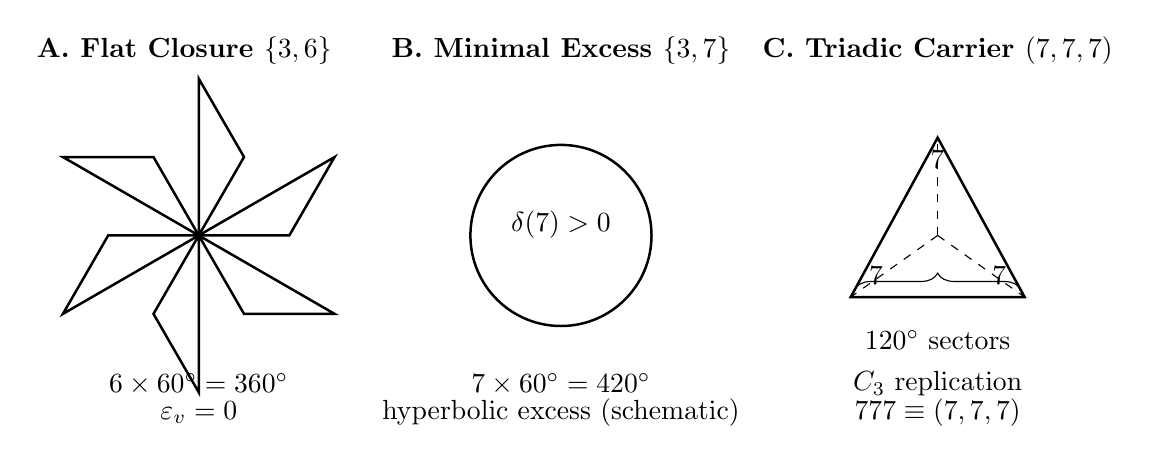
\begin{tikzpicture}[scale=0.92]
\node at (-5.2,2.55) {\textbf{A. Flat Closure $\{3,6\}$}};
\foreach \i in {0,60,...,300} {
    \draw[line width=0.9pt] (-5,0)
      -- ++(\i:1.25)
      -- ++(\i+60:1.25)
      -- cycle;
}
\node at (-5,-2.05) {$6\times 60^\circ = 360^\circ$};
\node at (-5,-2.45) {$\varepsilon_v=0$};

\node at (0,2.55) {\textbf{B. Minimal Excess $\{3,7\}$}};
\draw[line width=0.9pt] (0,0) circle (1.25);
\node at (0,0.15) {$\delta(7)>0$};
\node at (0,-2.05) {$7\times 60^\circ = 420^\circ$};
\node at (0,-2.45) {hyperbolic excess (schematic)};

\node at (5.2,2.55) {\textbf{C. Triadic Carrier $(7,7,7)$}};
\draw[line width=0.9pt] (4,-0.85) -- (6.4,-0.85) -- (5.2,1.35) -- cycle;
\draw[dashed] (5.2,0.0) -- (5.2,1.35);
\draw[dashed] (5.2,0.0) -- (4,-0.85);
\draw[dashed] (5.2,0.0) -- (6.4,-0.85);
\draw[decorate,decoration={brace,amplitude=6pt}]
  (4.05,-0.75) -- (6.35,-0.75)
  node[midway,yshift=-18pt] {$120^\circ$ sectors};
\node at (5.2,1.05) {$7$};
\node at (4.35,-0.55) {$7$};
\node at (6.05,-0.55) {$7$};
\node at (5.2,-2.05) {$C_3$ replication};
\node at (5.2,-2.45) {$777\equiv(7,7,7)$};
\end{tikzpicture}

\caption{From Euclidean closure $\{3,6\}$ to the minimal hyperbolic excess insertion $\{3,7\}$, replicated across the three symmetry sectors of the equilateral triangle under $C_3$.}
\end{figure}

\section*{Closing Remark}

The symbol $777$ denotes a classical boundary-selected curvature invariant:
the minimal hyperbolic excess integer ($k^\star=7$) replicated under the
threefold symmetry of the equilateral triangle.

\end{document}
